\documentclass[10pt, landscape, a4paper]{article}

\usepackage[utf8]{inputenc}
\usepackage{multicol}
\usepackage{calc}
\usepackage{ifthen}
\usepackage[landscape]{geometry}
\usepackage{amsmath}
\usepackage{graphicx}

\geometry{top=1cm,left=1cm,right=1cm,bottom=1cm}

% Turn off header and footer
\pagestyle{empty}


% Redefine section commands to use less space
\makeatletter
\renewcommand{\section}{\@startsection{section}{1}{0mm}%
                                {-1ex plus -.5ex minus -.2ex}%
                                {0.5ex plus .2ex}%x
                                {\normalfont\large\bfseries}}
\renewcommand{\subsection}{\@startsection{subsection}{2}{0mm}%
                                {-1explus -.5ex minus -.2ex}%
                                {0.5ex plus .2ex}%
                                {\normalfont\normalsize\bfseries}}
\renewcommand{\subsubsection}{\@startsection{subsubsection}{3}{0mm}%
                                {-1ex plus -.5ex minus -.2ex}%
                                {1ex plus .2ex}%
                                {\normalfont\small\bfseries}}
\makeatother

% Define BibTeX command
\def\BibTeX{{\rm B\kern-.05em{\sc i\kern-.025em b}\kern-.08em
    T\kern-.1667em\lower.7ex\hbox{E}\kern-.125emX}}

% Don't print section numbers
\setcounter{secnumdepth}{0}


\setlength{\parindent}{0pt}
\setlength{\parskip}{7pt}
% \setlength{\parskip}{0pt plus 0.5ex}


% -----------------------------------------------------------------------

\begin{document}

\raggedright
% \footnotesize
\small
\begin{multicols}{3}


% multicol parameters
% These lengths are set only within the two main columns
%\setlength{\columnseprule}{0.25pt}
\setlength{\premulticols}{1pt}
\setlength{\postmulticols}{1pt}
\setlength{\multicolsep}{1pt}
\setlength{\columnsep}{2pt}

\subsection{Funktioner}

{
  \renewcommand{\arraystretch}{2.4}
  \renewcommand{\tabcolsep}{5pt}
  \begin{tabular}{l|c|l}
    sin  &
    o/h &
    $\sin \theta = \cos \left(\dfrac{\pi}{2} - \theta \right) = \dfrac{1}{\csc \theta}$ \\
    \hline
    cos &
    a/h &
    $\cos \theta = \sin \left(\dfrac{\pi}{2} - \theta \right) = \dfrac{1}{\sec \theta}$ \\
    \hline
    tan &
    o/a &
    $\tan \theta = \dfrac{\sin \theta}{\cos \theta} = \cot \left(\dfrac{\pi}{2} - \theta \right) = \dfrac{1}{\cot \theta}$ \\
    \hline
    cot &
    a/o &
    $\cot \theta = \dfrac{\cos \theta}{\sin \theta} = \tan \left(\dfrac{\pi}{2} - \theta \right) = \dfrac{1}{\tan \theta}$ \\
    \hline
    sec &
    h/a &
    $\sec \theta = \csc \left(\dfrac{\pi}{2} - \theta \right) = \dfrac{1}{\cos \theta}$ \\
    \hline
    csc &
    h/a &
    $\csc \theta = \sec \left(\dfrac{\pi}{2} - \theta \right) = \dfrac{1}{\sin \theta}$
  \end{tabular}
}

\subsection{Satser}
\textit{Sinussatsen}
\begin{equation*}
  \frac{\sin \alpha}{a} = \frac{\sin \beta}{b} = \frac{\sin \gamma}{c}
\end{equation*}
\textit{Cosinussatsen}
\begin{align*}
  a^2 &= b^2+c^2-2bc\cdot\cos(\alpha) \\
  b^2 &= a^2+c^2-2ac\cdot\cos(\beta) \\
  c^2 &= a^2+b^2-2ab\cdot\cos(\gamma)
\end{align*}
\textit{Areasatsen}
\begin{equation*}
  \frac{ab \sin \gamma}{2} = \frac{ac \sin \beta}{2} = \frac{bc \sin \gamma}{2}
\end{equation*}
\textit{Hjälpvinkelmetoden}
\begin{align*}
  & a \sin x + b \cos x = \\
  &= \sqrt{a^2+b^2} \sin \left(x + \arcsin\left(\frac{b}{\sqrt{a^2+b^2}}\right)\right) \\
  &= \sqrt{a^2+b^2} \sin \left(x + \arccos\left(\frac{a}{\sqrt{a^2+b^2}}\right)\right)
\end{align*}
\textit{Identiteter}
\begin{align*}
  (\sin x)^2 + (\cos x)^2 &= 1 \\
  (\sec x)^2 - (\tan x)^2 &= 1 \\
  (\csc x)^2 - (\cot x)^2 &= 1
\end{align*}

\subsection{Vinklar}

{
  \renewcommand{\arraystretch}{2.4}
  \renewcommand{\tabcolsep}{5pt}
  \begin{tabular}{l|ccccccc}
    &
    $0$ &
    $\dfrac{\pi}{12}$ &
    $\dfrac{\pi}{6}$ &
    $\dfrac{\pi}{4}$ &
    $\dfrac{\pi}{3}$ &
    $\dfrac{5\pi}{12}$ &
    $\dfrac{\pi}{2}$ \\
    \hline
    $\sin$ &
    $0$ &
    $\dfrac{\sqrt{6}-\sqrt{2}}{4}$ &
    $\dfrac{1}{2}$ &
    $\dfrac{\sqrt{2}}{2}$ &
    $\dfrac{\sqrt{3}}{2}$ &
    $\dfrac{\sqrt{6}+\sqrt{2}}{4}$ &
    $1$ \\
    \hline
    $\cos$ &
    $1$ &
    $\dfrac{\sqrt{6}+\sqrt{2}}{4}$ &
    $\dfrac{\sqrt{3}}{2}$ &
    $\dfrac{\sqrt{2}}{2}$ &
    $\dfrac{1}{2}$ &
    $\dfrac{\sqrt{6}-\sqrt{2}}{4}$ &
    $0$ \\
    \hline
    $\tan$ &
    $0$ &
    $2-\sqrt{3}$ &
    $\dfrac{\sqrt{3}}{3}$ &
    $1$ &
    $\sqrt{3}$ &
    $2+\sqrt{3}$ &
    $\infty$ \\
    \hline
    $\cot$ &
    $\infty$ &
    $2+\sqrt{3}$ &
    $\sqrt{3}$ &
    $1$ &
    $\dfrac{\sqrt{3}}{3}$ &
    $2-\sqrt{3}$ &
    $0$ \\
    \hline
    $\sec$ &
    $1$ &
    $\sqrt{6} - \sqrt{2}$ &
    $\dfrac{2\sqrt{3}}{3}$ &
    $\sqrt{2}$ &
    $2$ &
    $\sqrt{6}+\sqrt{2}$ &
    $\infty$ \\
    \hline
    $\csc$ &
    $\infty$ &
    $\sqrt{6}+\sqrt{2}$ &
    $2$ &
    $\sqrt{2}$ &
    $\dfrac{2\sqrt{3}}{3}$ &
    $\sqrt{6} - \sqrt{2}$ &
    $1$
  \end{tabular}
}

\subsection{Vinkeltransformationer}
\textit{Addition}
\begin{align*}
  \sin (\alpha \pm \beta) &= \sin \alpha \cos \beta \pm \cos \alpha \sin \beta \\
  \cos (\alpha \pm \beta) &= \cos \alpha \cos \beta \mp \sin \alpha \sin \beta \\
  \tan(\alpha \pm \beta)  &= \frac{\tan \alpha \pm \tan \beta}{1 \mp \tan \alpha \tan \beta}
\end{align*}
\textit{Halva vinkeln}
\begin{align*}
  \sin \frac{\theta}{2} &= \pm \sqrt{\frac{1-\cos \theta}{2}}
  &
  \cos \frac{\theta}{2} &= \pm \sqrt{\frac{1+\cos \theta}{2}}
\end{align*}
\begin{align*}
  \tan \frac{\theta}{2} = \csc\theta - \cot\theta = \frac{\sin\theta}{1+\cos\theta} = \frac{1-\cos\theta}{\sin\theta}
\end{align*}
\textit{Dubbla vinkeln}
\begin{align*}
  \sin 2\theta &= 2 \sin \theta \cos \theta \\
  \cos 2\theta &= (\cos \theta)^2 - (\sin \theta)^2 \\
  \tan 2\theta &= \frac{2\tan\theta}{1-(\tan\theta)^2}
\end{align*}
\textit{Trippla vinkeln}
\begin{align*}
  \sin 3\theta &= 3 (\cos\theta)^2 \sin\theta - (\sin\theta)^2 \\
  &= 3\sin \theta - 4(\sin \theta)^3 \\
  \cos 3\theta &= (\cos\theta)^3 - 3(\sin\theta)^2\cos\theta \\
  &= 4(\cos \theta)^3 + -3\cos \theta
\end{align*}

\subsection{Arcusfunktionerna}
\begin{align*}
  \sin^{-1} x + \cos^{-1} x &= \pi/2 \\
  \tan^{-1} x + \cot^{-1} x &= \pi/2 \\
  \tan^{-1} x + \tan^{-1} 1/x &= \begin{cases} \pi/2 & \mbox{if }x > 0 \\  -\pi/2 & \mbox{if }x < 0 \end{cases}
\end{align*}
\begin{align*}
  \sin[\arccos(x)] &= \sqrt{1-x^2} &
  \tan[\arcsin (x)] &= \dfrac{x}{\sqrt{1 - x^2}} \\
  \sin[\arctan(x)] &= \dfrac{x}{\sqrt{1+x^2}} &
  \tan[\arccos (x)] &= \dfrac{\sqrt{1 - x^2}}{x} \\
  \cos[\arctan(x)] &= \dfrac{1}{\sqrt{1+x^2}} &
  \cot[\arcsin (x)] &= \dfrac{\sqrt{1 - x^2}}{x} \\
  \cos[\arcsin(x)] &= \sqrt{1-x^2} &
  \cot[\arccos (x)] &= \dfrac{x}{\sqrt{1 - x^2}}
\end{align*}

\subsection{Enhetscirkeln med standardvinklar}
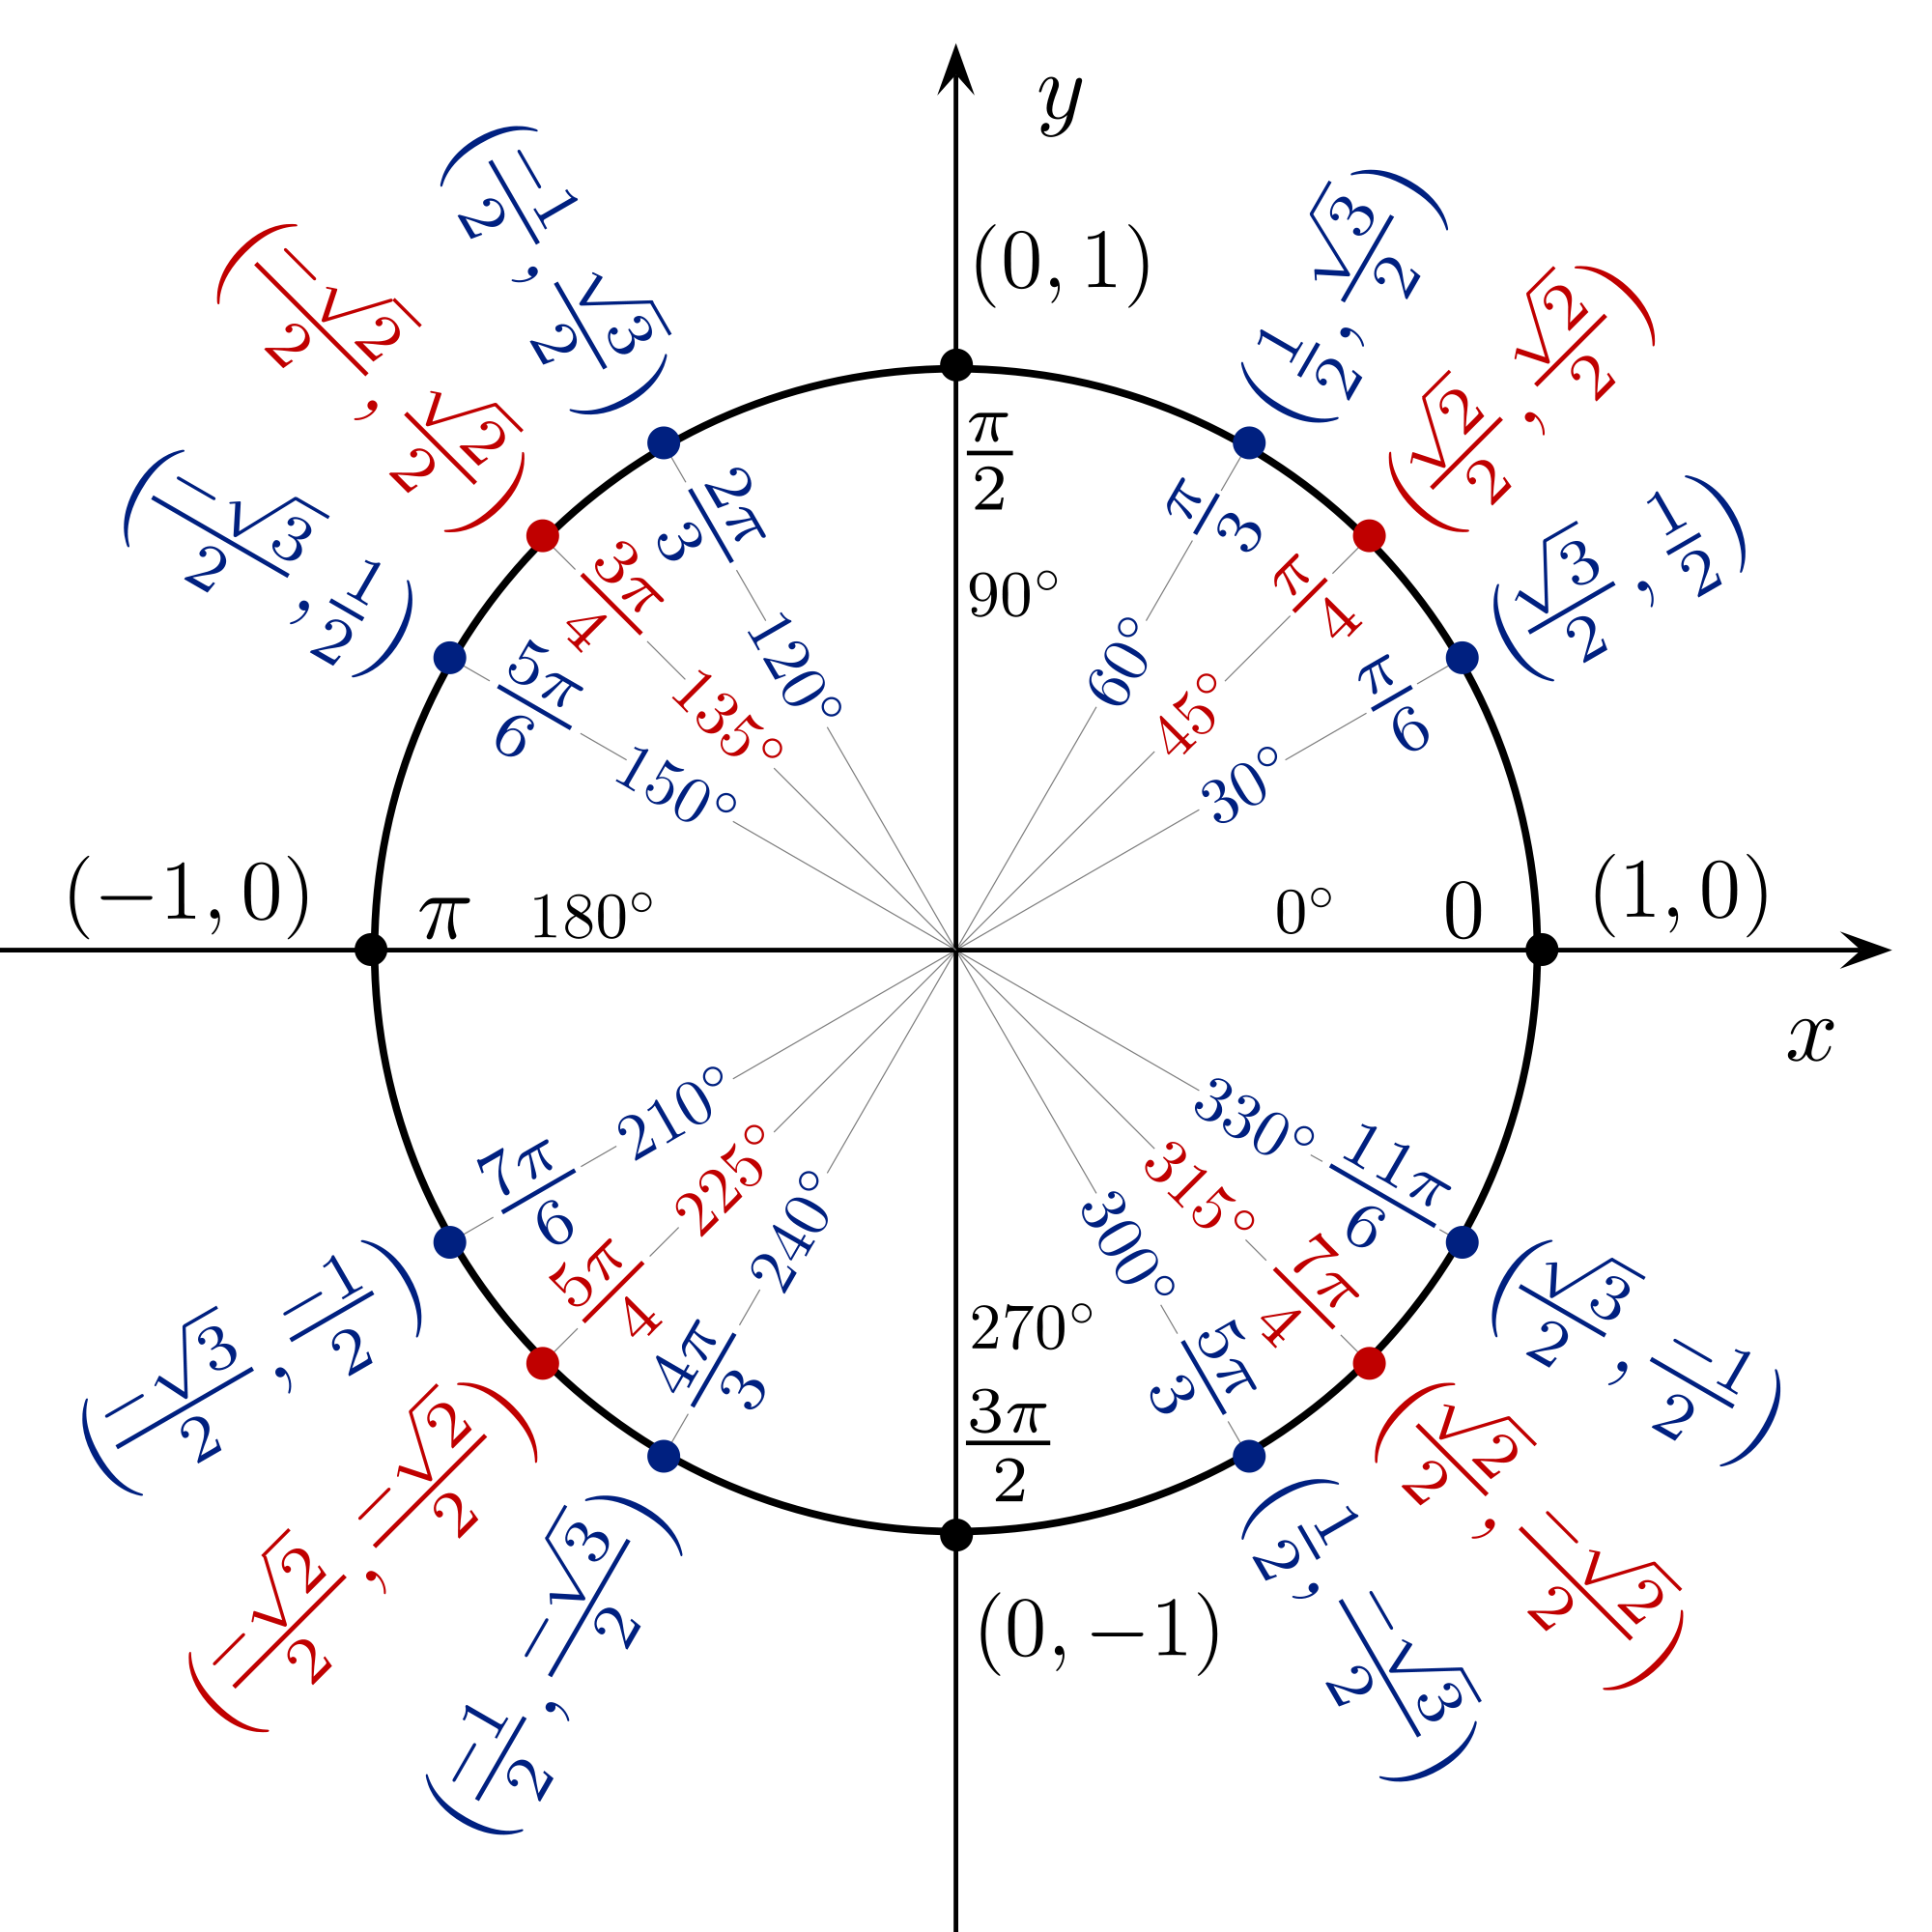
\includegraphics[width=8cm]{2000px-Unit_circle_angles_color-svg.png}

\rule{0.33\linewidth}{0.25pt}
\\
%\scriptsize
\tiny
Trigonometri Referens, \texttt{trigref.pdf} v. 0.1
\\
Viktor Qvarfordt -- \today

\end{multicols}
\end{document}